%\documentclass[11pt]{article}
%\usepackage{fullpage}

%\begin{document}

\subsection{Overview}
This section provides a detailed view over the system architecture and its components, describing them at both logical and physical level. \newline

\textbf{Section 2.2 - High-level components}: This subsection provides a description of high-level components and their interactions. \newline

\textbf{Section 2.3 - Component view}: This subsection provides a detailed insight of the components described in the previous section. \newline

\textbf{Section 2.4 - Deployment view}: This subsection provides a set of indications on how to deploy the illustrated components on physical tiers. \newline

\textbf{Section 2.5 - Runtime view}: In this subsection sequence diagrams are used to describe the way components interact to accomplish specific tasks typically related to your use cases. \newline

\textbf{Section 2.6 - Component interfaces}: This subsection provides a description of the different type of interfaces among the various described components. \newline

\textbf{Section 2.7 - Selected architectural styles and patterns}: This subsection provides a list of the architectural styles, design patterns and paradigms adopted in the design phase. \newline

\textbf{Section 2.8 - Other design decisions}: This subsection lists of all other relevant design decisions that were not mentioned before.

\clearpage

\subsection{High-level components}
The main high-level components of the system are:

\begin{itemize}
\item \textbf{Database}: The system data layer; it includes all structures and entities responsible for data storage and management. No application logic is found at this level, apart from the DBMS one that must guarantee the correct functioning of the data structures while assuring the ACID properties of transactional databases.

\item \textbf{Application Server}: This layer encloses all the logic for the system applications, including the logic needed to interface with external systems and the key algorithms.

\item \textbf{Mobile App Interface}: The client layer dedicated to mobile devices; it communicates directly with the Application Server and only includes presentation logic.

\item \textbf{Wearable App Interface}: The client layer dedicated to wearable devices equipped with WearOS (Android) and watchOS (Apple). The app requires to be installed also on a smartphone and to be paired via bluetooth. It just shows dinamically user's data.

\item \textbf{Script Interface}:  The client layer dedicated to third parties who need to get huge quantities of data: our application doesn't provide other visual interfaces besides the mobile one, but we allow companies to get data through scripts and HTTPS requests providing them libraries to include in order to allow the communication (authentication always required). The layer communicates directly with the Application Server.
\end{itemize}

The described components are structured in three layers, as shown in the following figure. It also includes the interaction with external systems, that is intended to happen at the level of the Application Server.

\begin{center}
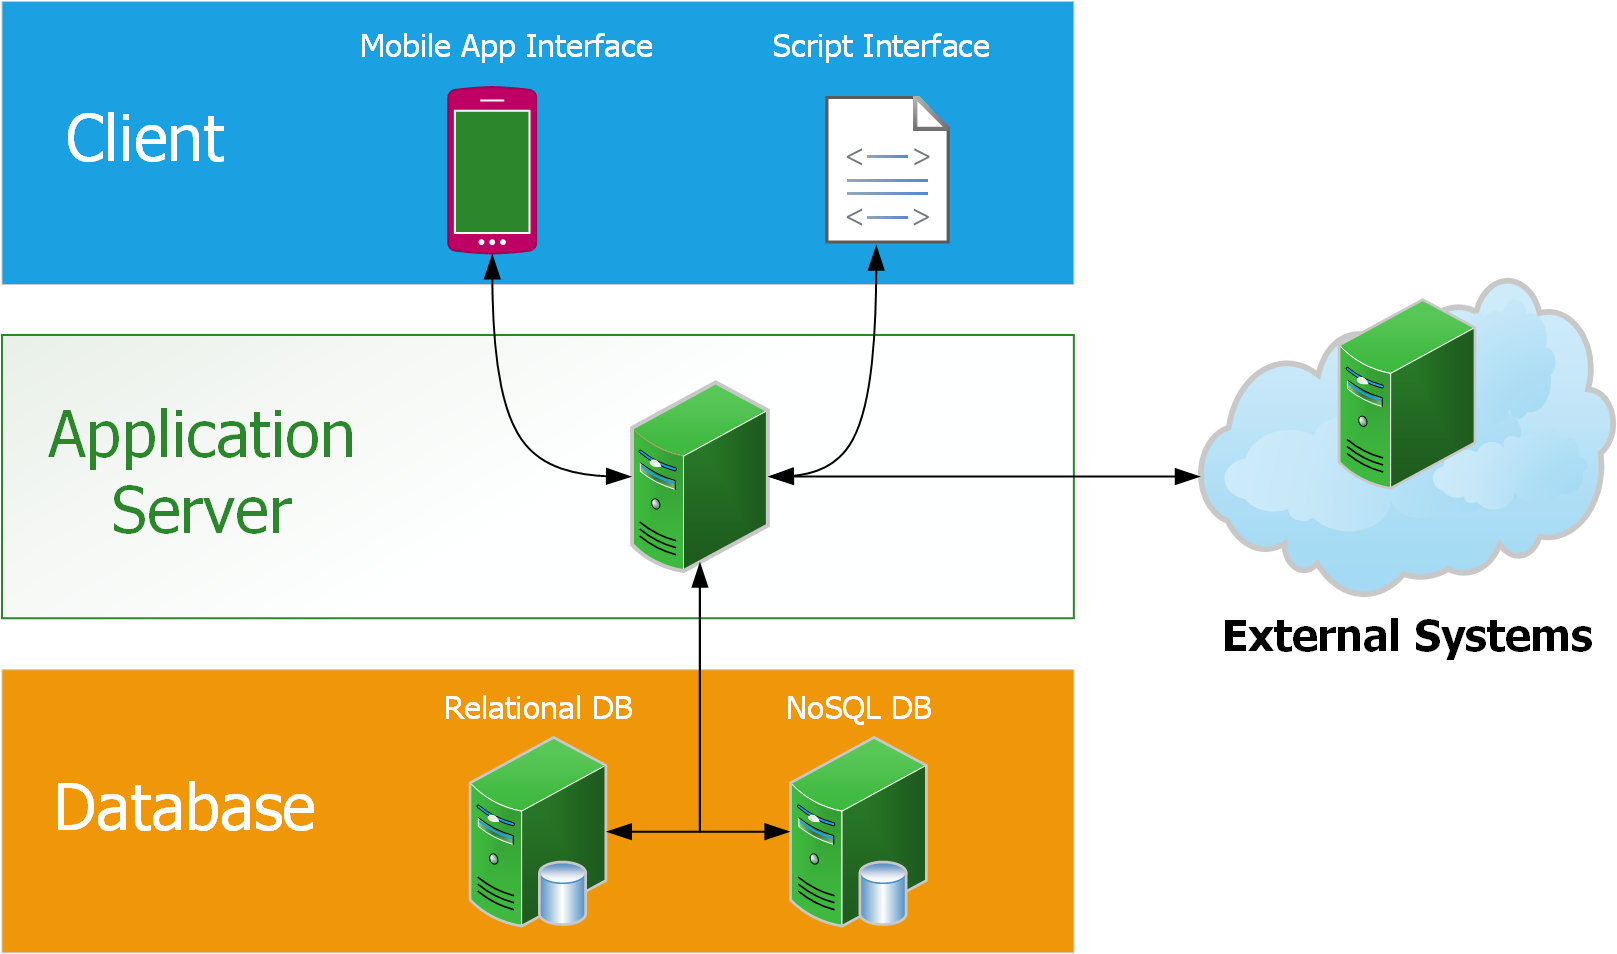
\includegraphics[scale=0.69]{sections/diagrams/layers.png}
\newline
\captionof{figure}{Logical layers of the system}
\end{center}

External systems are shown more in detail in the following figure: an high-level overview of the system components.

\begin{center}
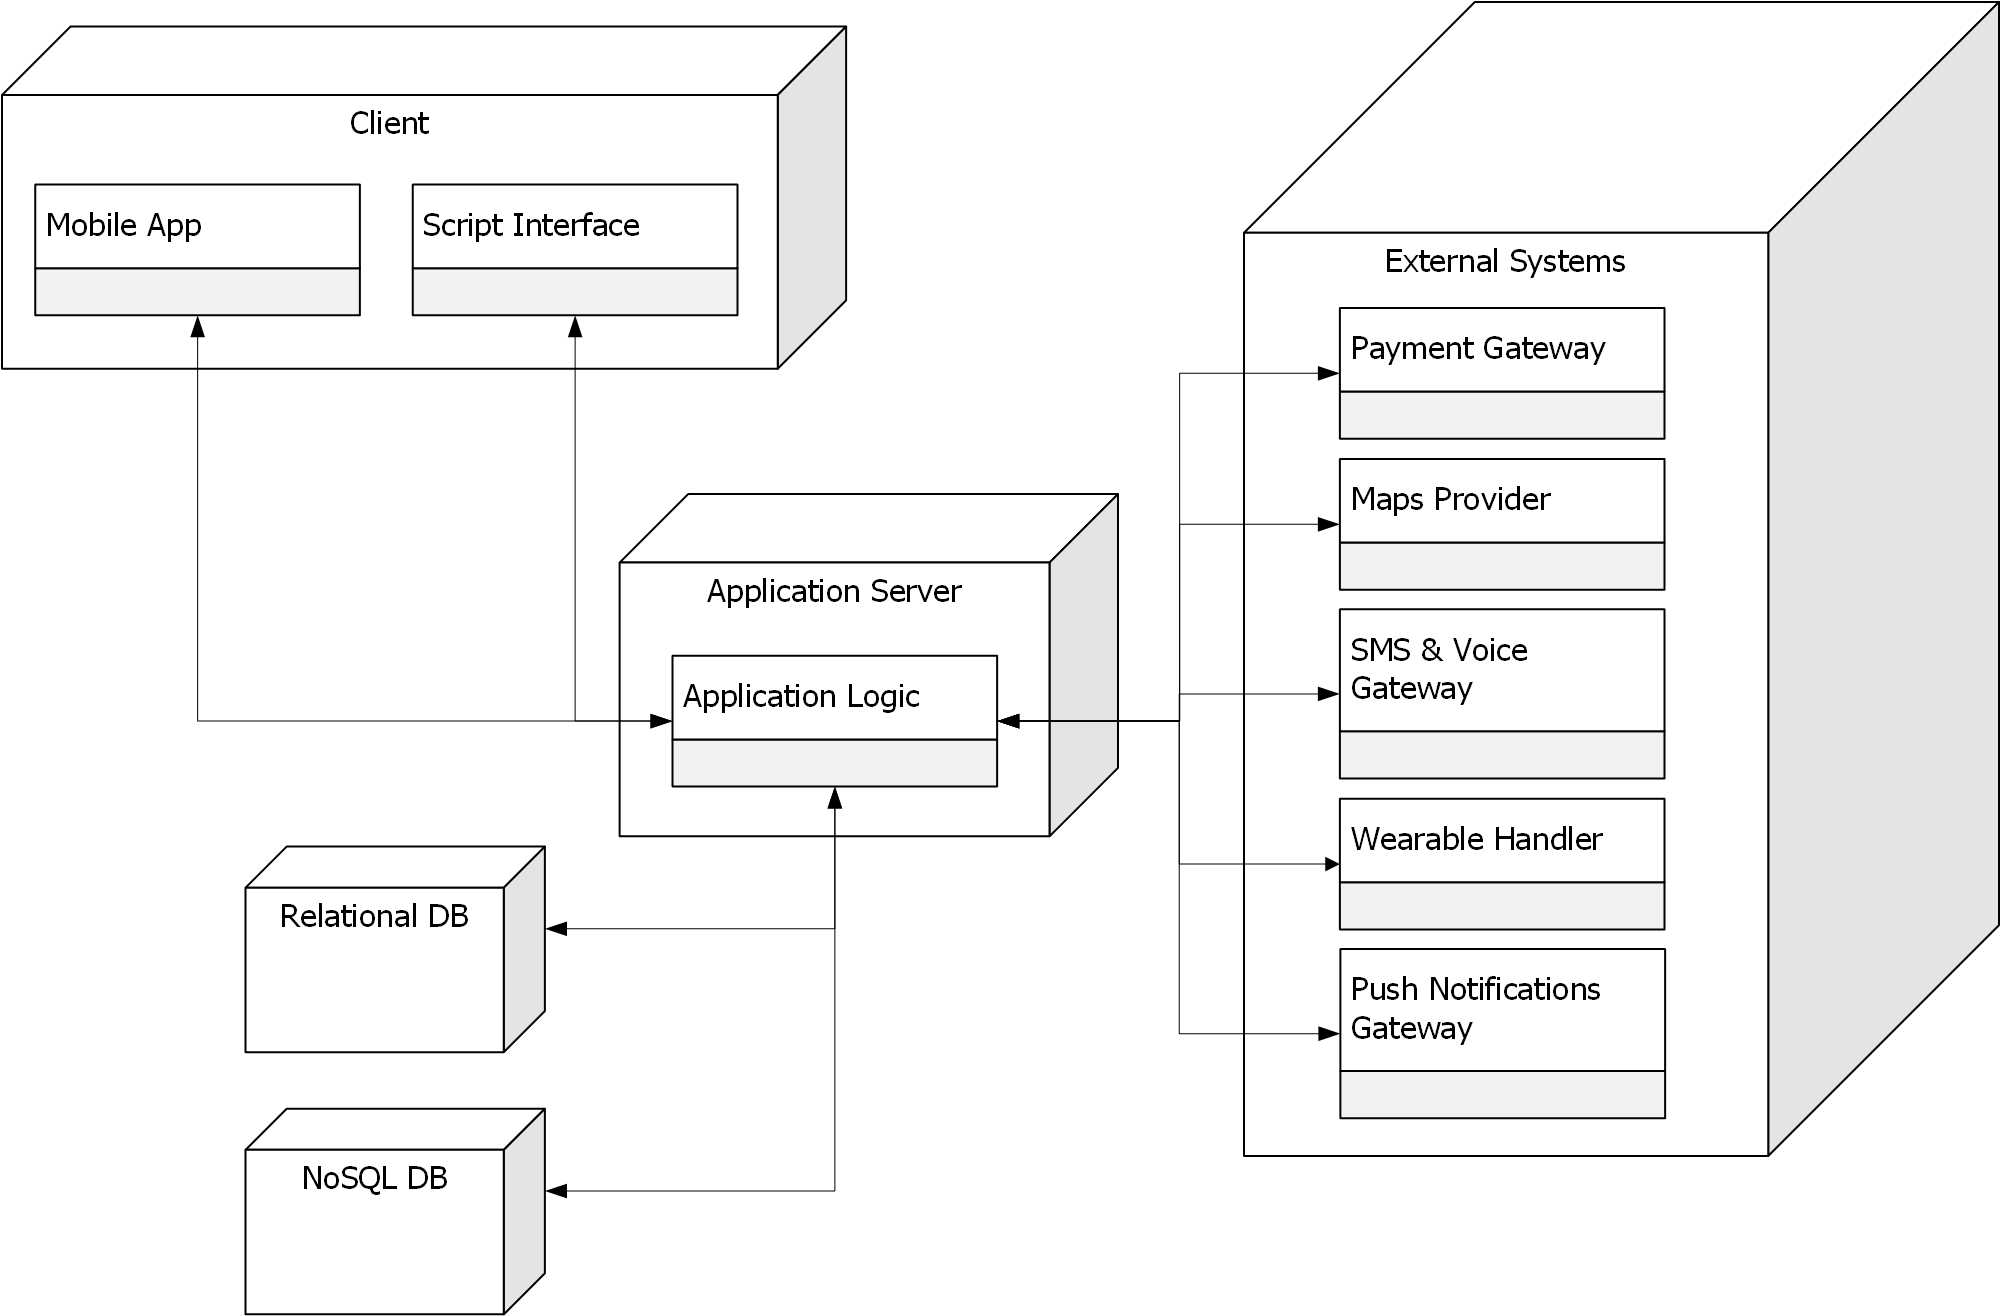
\includegraphics[scale=0.6]{sections/diagrams/highlevel.png}
\newline
\captionof{figure}{High-level components of the system}
\end{center}

\subsection{Component view}
\subsubsection{Database}
The Database layer must only be accessible through the Application Server via a dedicated interface. With respect to this, the Application Server must provide a persistence unit to handle the dynamic behaviour of all of the persistent application data. \newline

Besides the Database Engines, this layer is composed by a DBMS, which is in main part relational. The relational approach offers advantages ranging from the easy extensibility to independency from the physical organization, and in general the ACID properties of its transactions. For all these reasons fixed in front data and those that change less frequently are committed to the RDBMS, while for the others a NoSQL is provided. In fact thanks to its well-known scalability it fits better for data accumulated in large numbers every second, which is the case of all the data collected by the application through the wearable device. \newline

The Database layer has to store all the data shown in the following ER diagram, the sensible of which must be encrypted before being stored.

\begin{center}
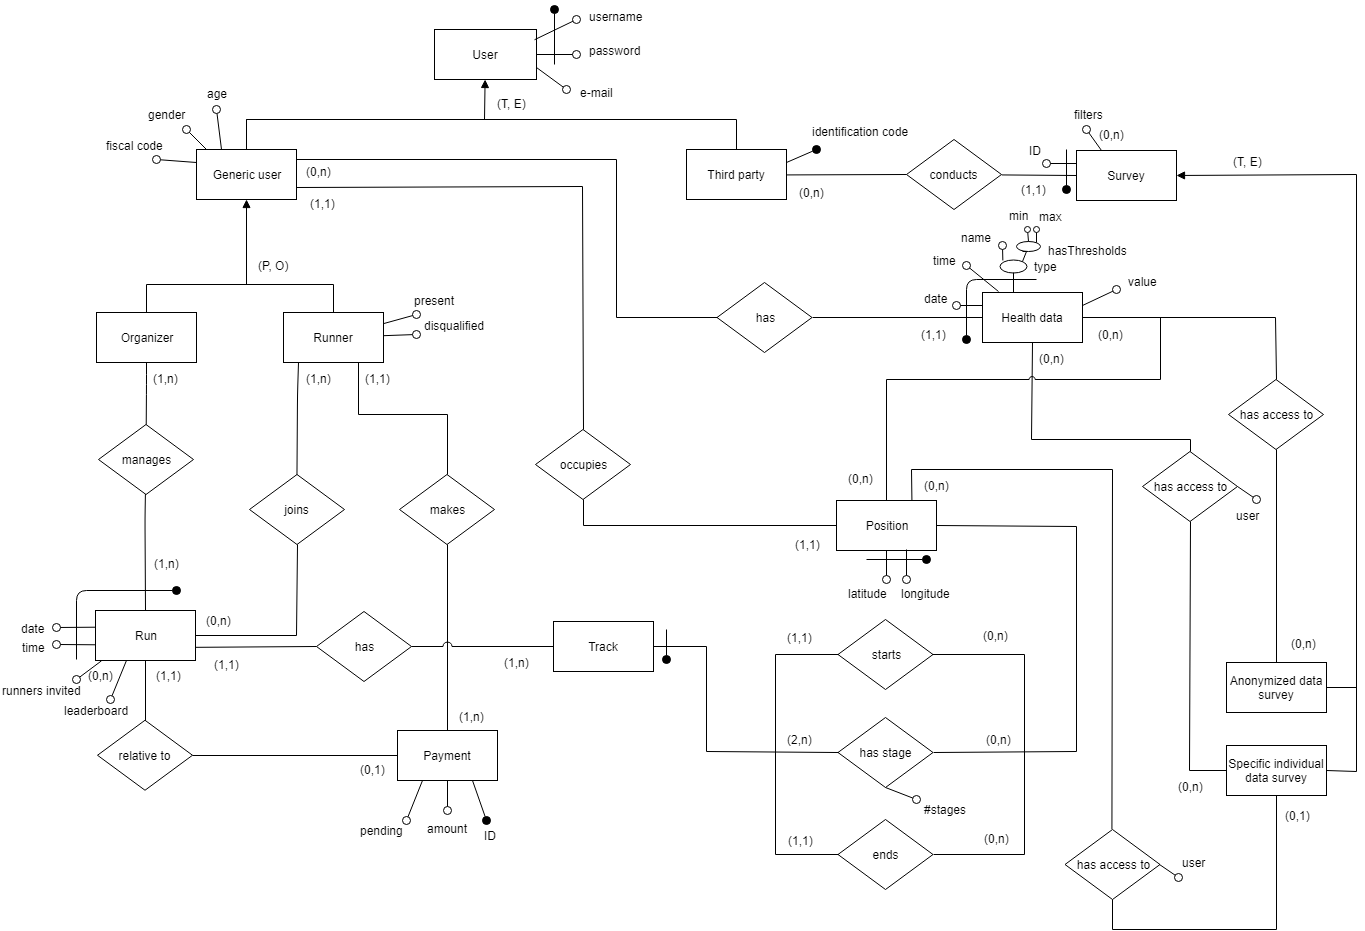
\includegraphics[scale=0.34]{sections/diagrams/ER.png}
\newline
\captionof{figure}{ER model of the system}
\end{center}

\subsubsection{Application Server}
This layer must handle the business logic as a whole, the connections with the Database Layer and the multiple ways of accessing the application from different clients and external systems. The main feature of the Application Server are the specific modules of business logic, which describe business rules and work-flows for each of the functionalities provided by the application itself. \newline

The interface with the data layer must be handled, as stated before, by a dedicated persistence unit, that will be in charge of the object-relation mapping and dynamic data access and management; this ensures the fact that only the Application Server can access the Database. \newline

The Application Server must provide a means to interface with the mobile clients via specific APIs in order to decouple the different layers with respect to their individual implementation. Moreover, it must provide a way to communicate with external systems by adapting the application to the existing external infrastructures. \newline

The main business logic modules must include:
\begin{itemize}
\item \textbf{UserManager}: This module manages all the logic involved with user account management, login, registration and profile customization, as well as the generation and provision of user credentials.

\item \textbf{DataHandler}: This module manages the logic needed to manage data requests from third parties. It also includes the logic needed to communicate with external wearable devices and get data from them. It must also serve as an interface with the external Wearable Handler (e.g. Health app for iOS, Google Fit for Android, other available apps from various manufacturers).

\item \textbf{MapManager}: This module includes the logic needed to correctly visualize maps and markers moving on them, and also allows to choose and visualize stages. It must also serve as an interface with the external Maps Provider.

\item \textbf{PaymentGateway}: The logic involved in the computation of final charges is included in this module; moreover, this unit must stand as an interface with the external Payment Gateway upon the act of the automatic payments.

\item \textbf{EmergencyManager}: This module includes the logic needed to manage emergency calls and the sending of SMS. It must also serve as an interface with the external SMS \& Voice Gateway.

\item \textbf{NotificationManager}: This module serves as a gateway from the UserManager module, which needs to send an email to the clients, by managing the logic behind the email notification services. It also manages the logic needed to send and receive push notifications serving as an interface with the external Push Notifications Gateway.

\item \textbf{RunManager}: This module allows users to observe, participate, create and manage running races. It also has to provide and show info about races and it gets data from the MapManager, used to update leaderboards.
\end{itemize}

\subsubsection{Mobile Application Client}
As stated in the RASD document, the Mobile Application Client represents the main interface for customers and it should be implemented for both Android and iOS.

The mobile application must be designed in a way that makes communications with the Application Server easy and independent from the implementation of both sides. In order to do so, adequate APIs must be defined and used similarly to what has been described for the interactions between the two server layers.

The mobile application UI must be designed following the guidelines provided by the Android and iOS producers.

The mobile application directly communicates with the business logic using its RESTful API interfaces.

\subsubsection{Wearable Application Client}
As stated in the RASD document, the Wearable Application Client should be implemented for both WearOS and watchOS.

The software module to be included in the application must manage the GPS locations of the device and the connection with the device sensors, as well as the transmission of all health data to the mobile application via bluetooth.

\subsubsection{Desktop Client}
As mentioned before, currently TrackMe doesn't offer a desktop or web version of its application. However, companies can get data through scripts and HTTPS requests using provided libraries to include in order to allow the communication (authentication always required).

The Desktop Client directly communicates with the business logic of the Application Server.

\begin{center}
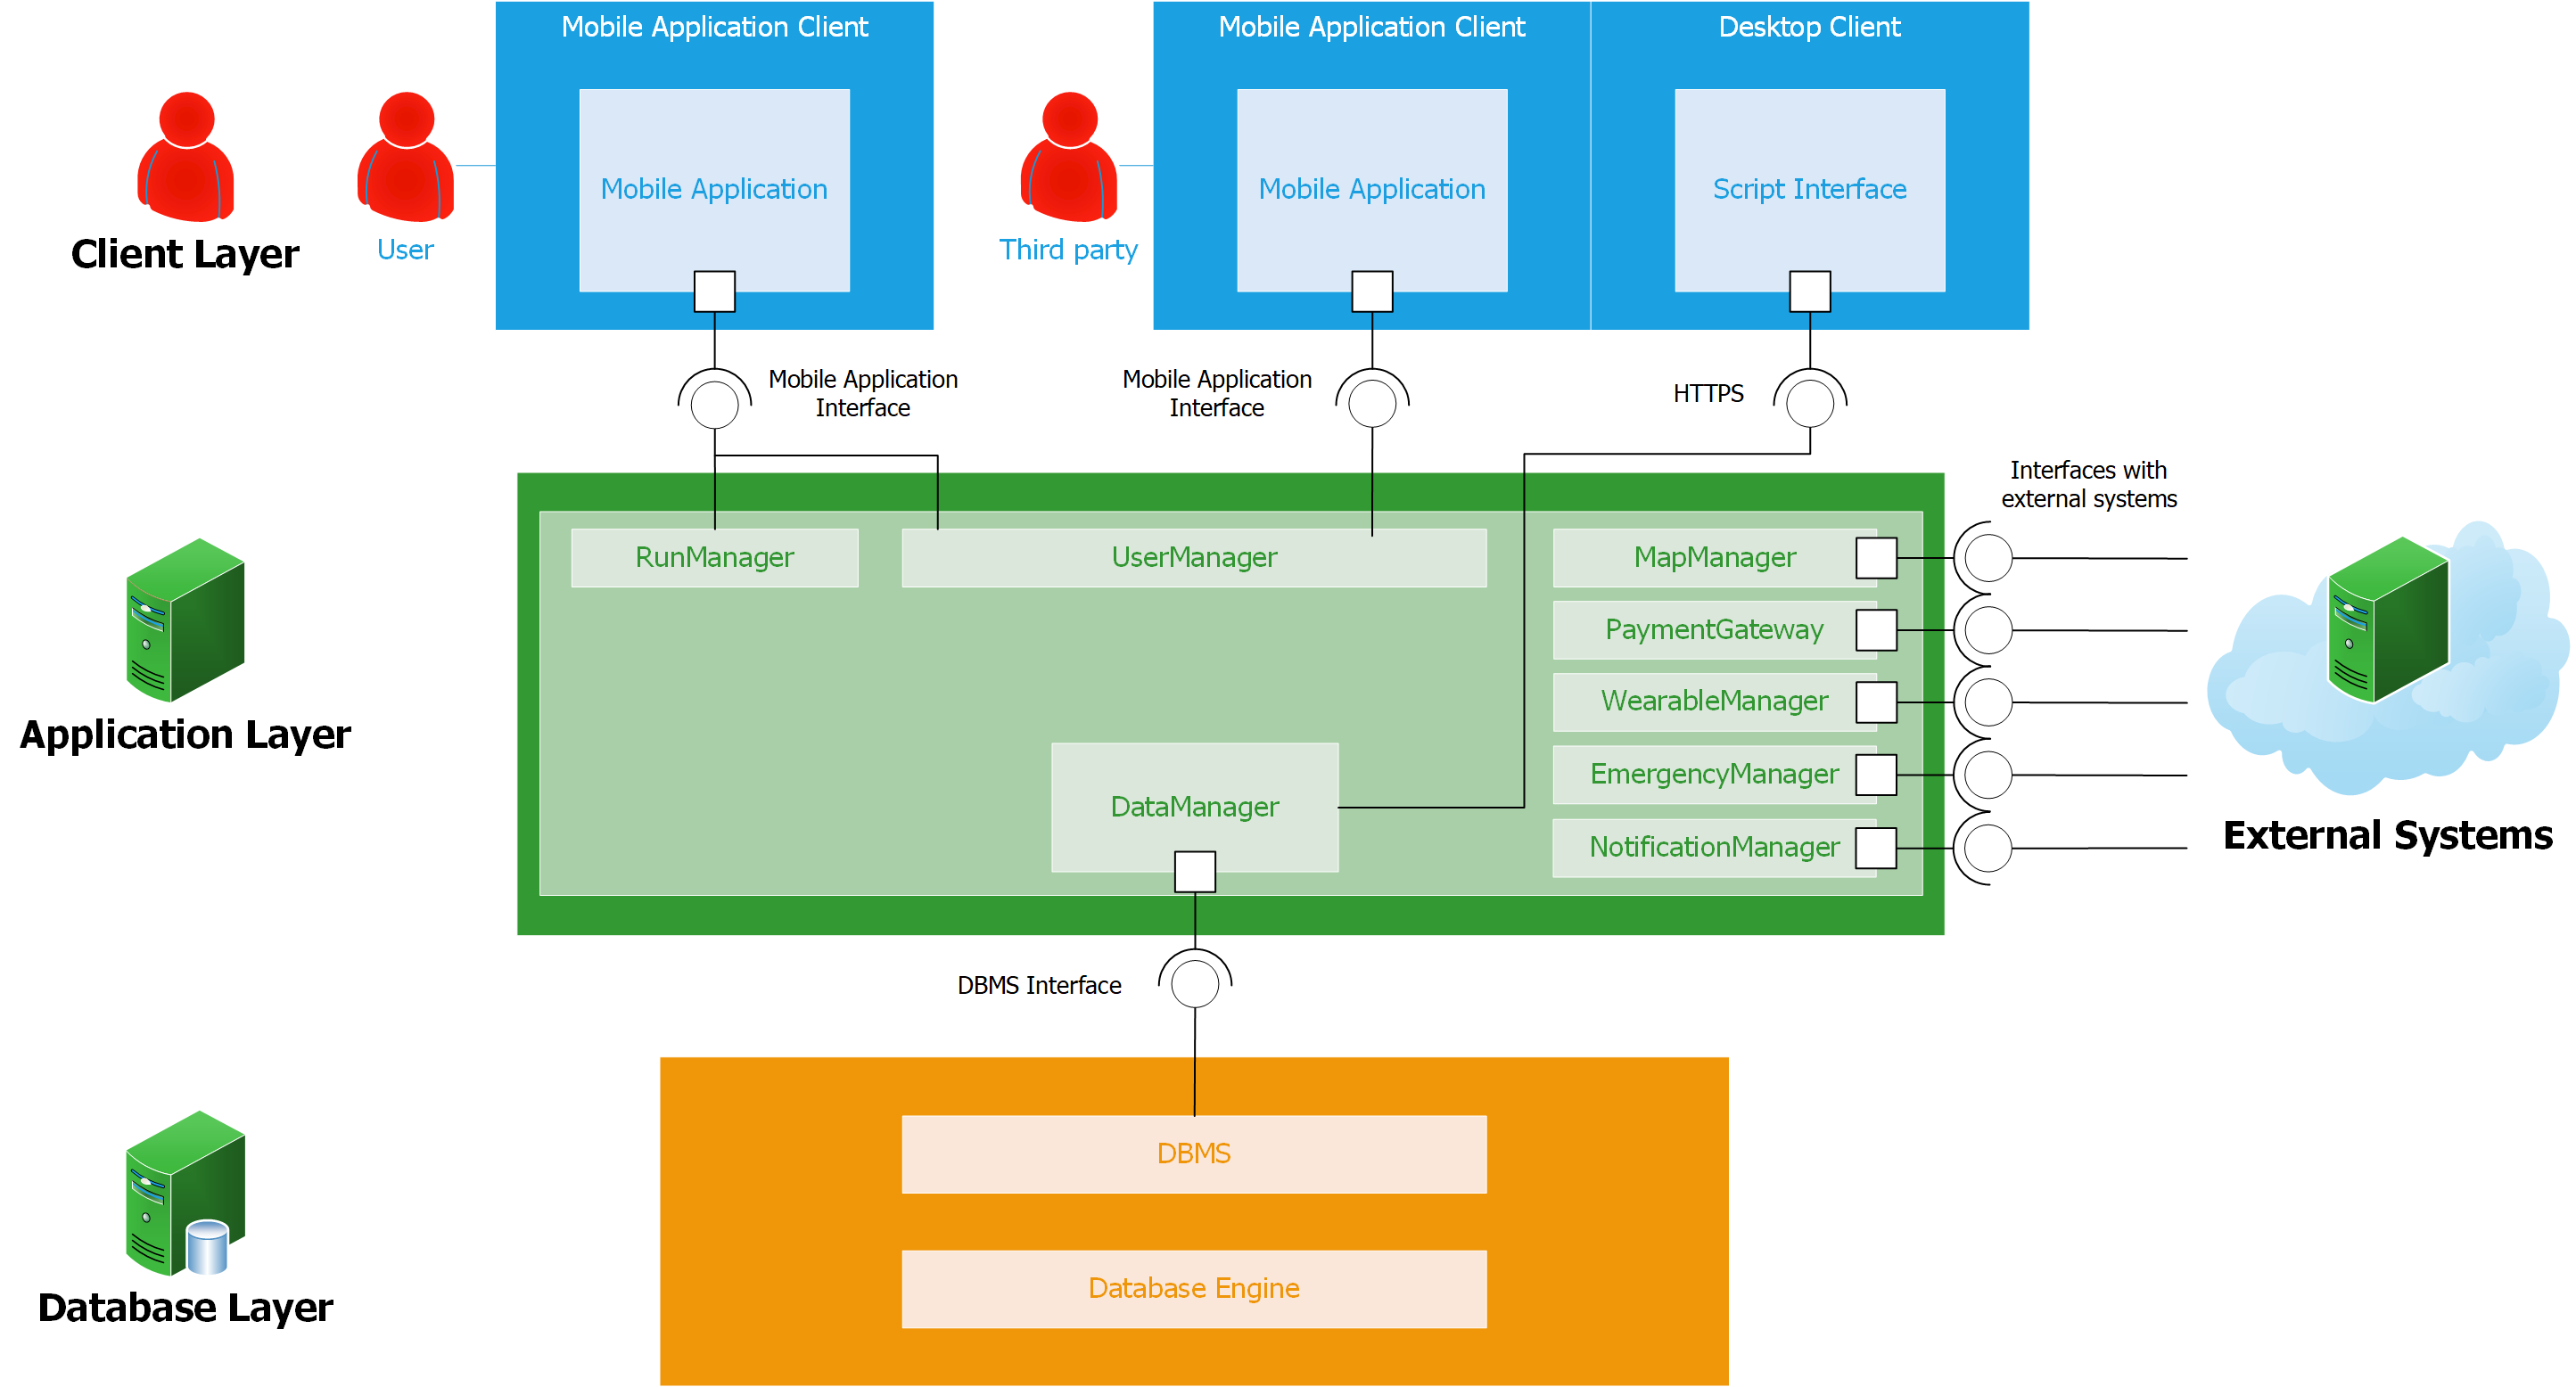
\includegraphics[scale=0.43]{sections/diagrams/globalCV.png}
\newline
\captionof{figure}{Global component view of the system}
\end{center}

\subsection{Deployment view}
The physical deployment of the system is done on 3 layers:
\begin{itemize}
\item Clients are deployed on different devices: the Desktop Device is related exclusively to third parties, the Mobile Device can be used by both third parties and generic users, the Wearable Device is related exclusively to generic users.

\item  The main logic of the application will be deployed in the Application Server. This server will communicate with all the other nodes - it will gather information from the external services (not here represented), manage user accounts and saved data from the Database and take requests and send back responses to the users.

\item The relational and the NoSQL databases can be deployed on the same physical machine. However, since they are completely independent one from the other, they could be moved on different machines as soon as it will be required for some reason.
\end{itemize}

\begin{center}
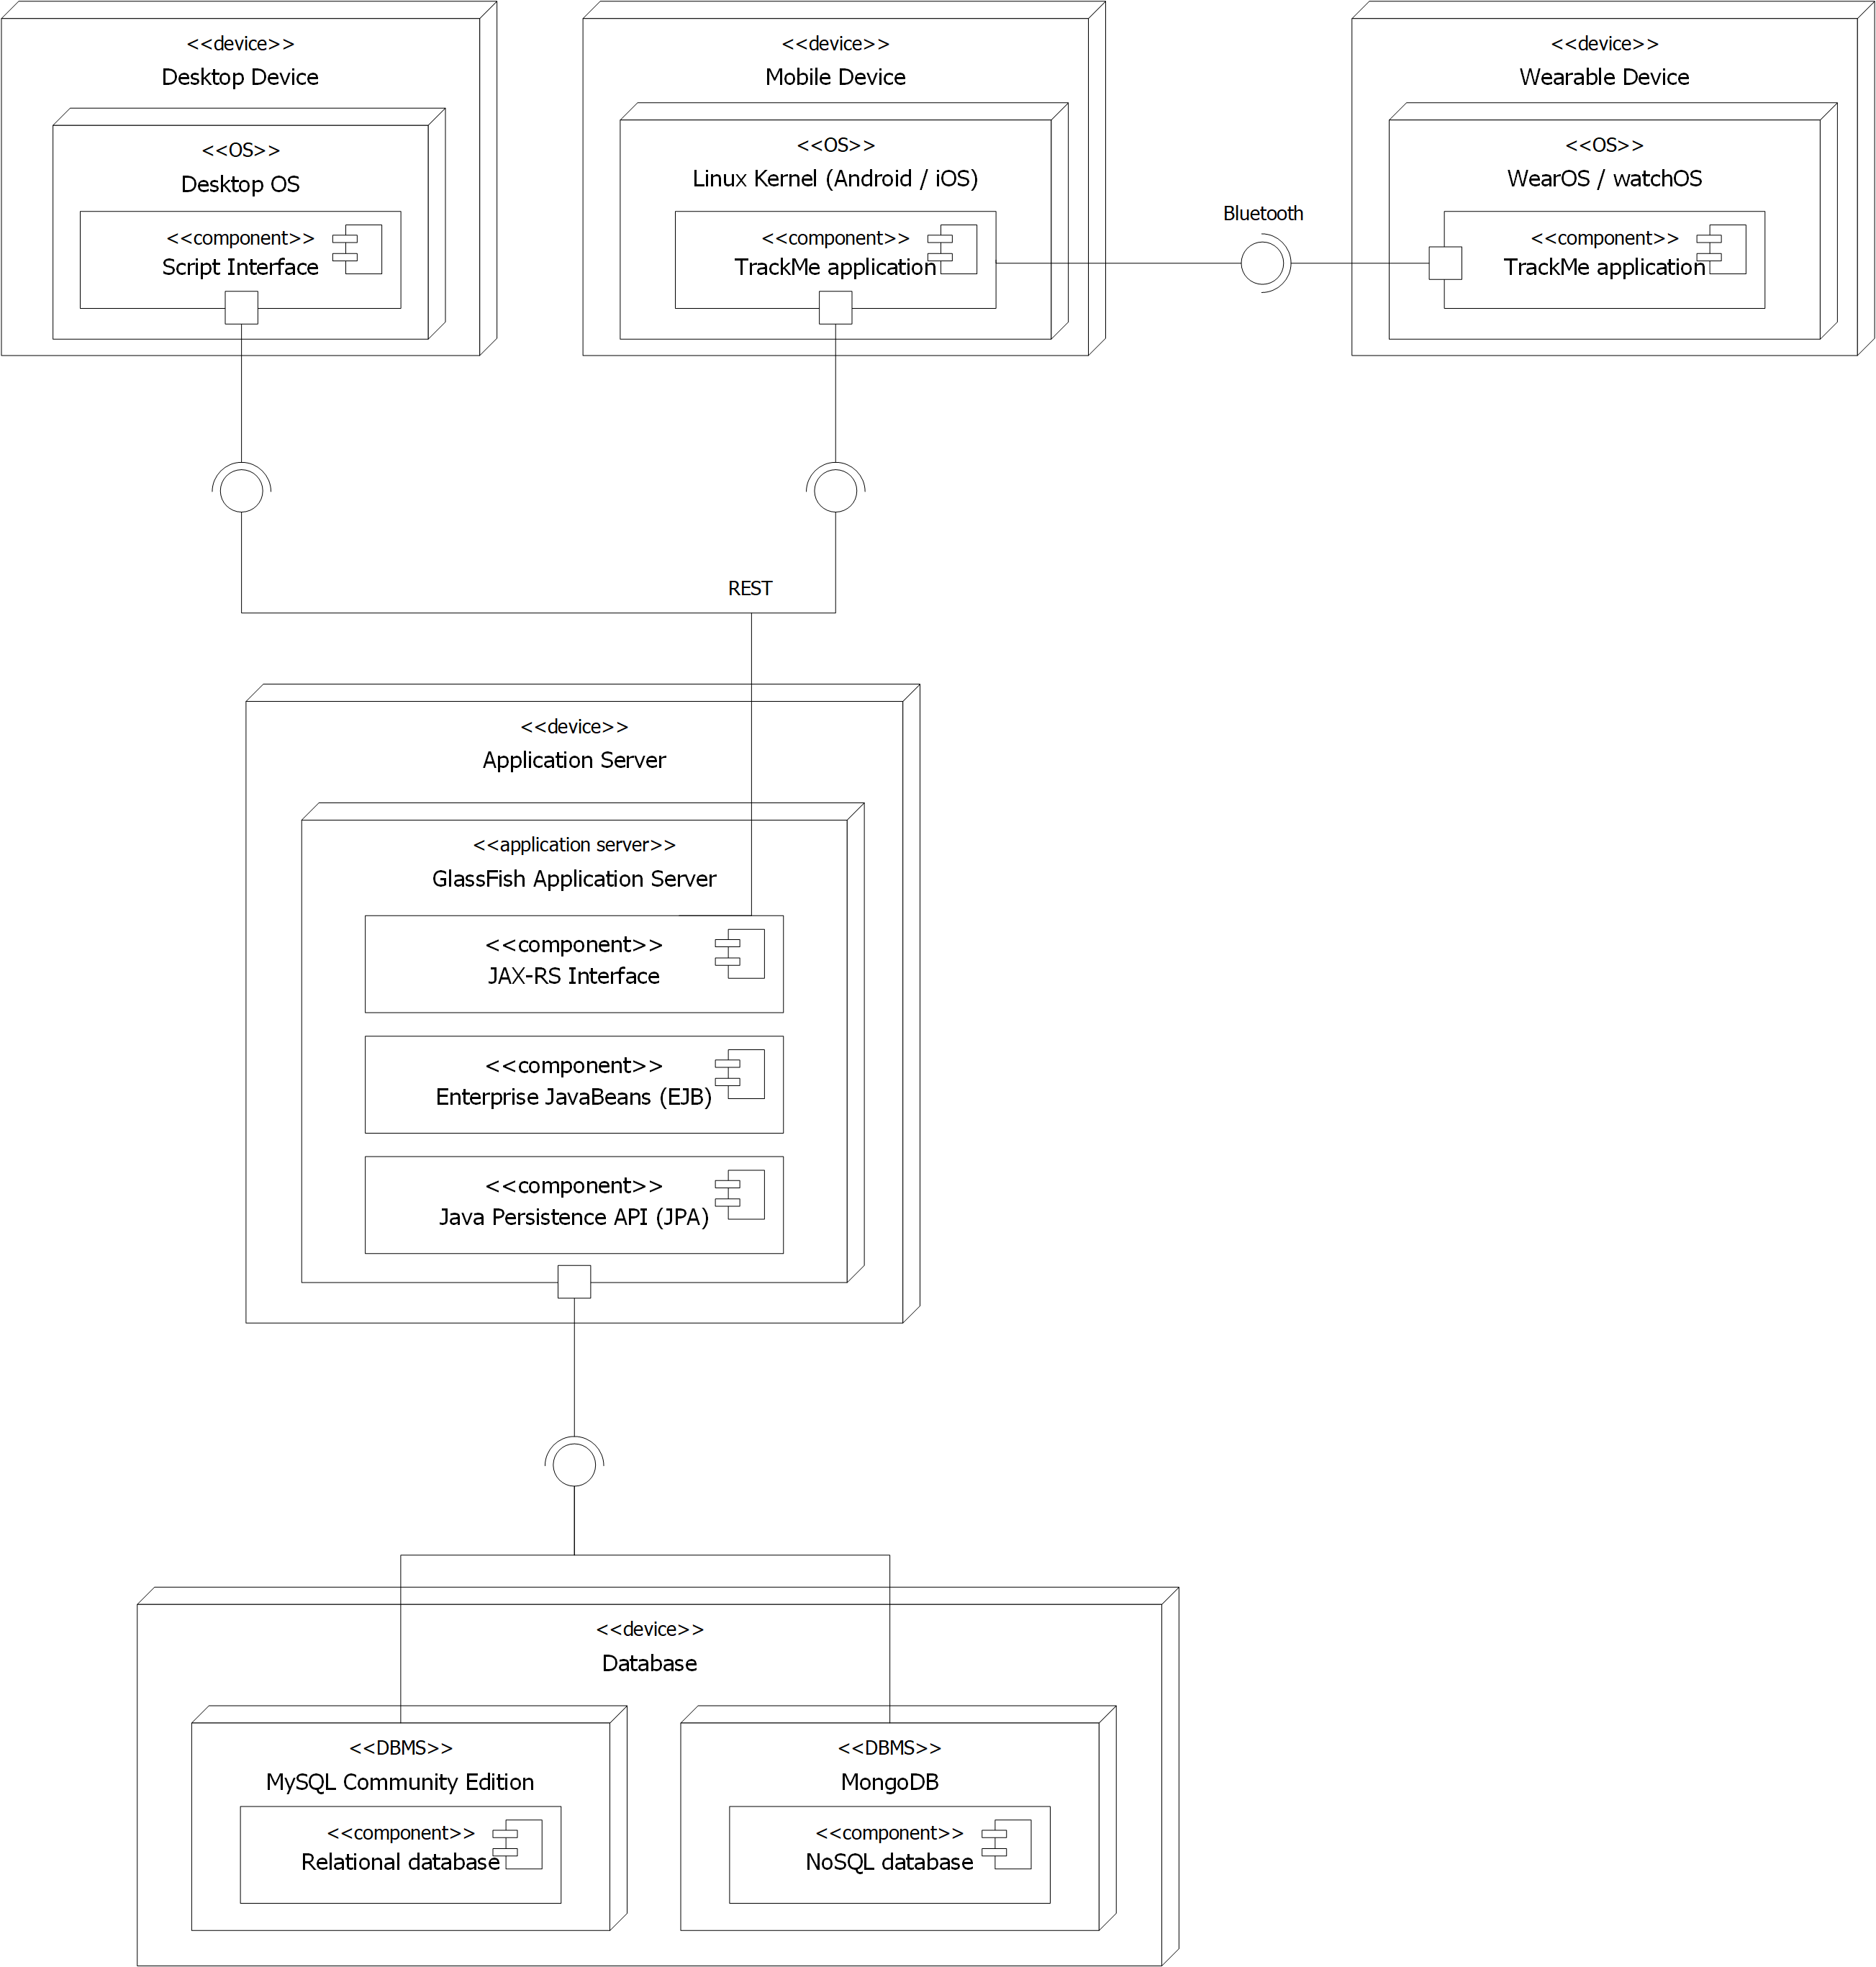
\includegraphics[scale=0.5]{sections/diagrams/deployment.png}
\newline
\captionof{figure}{Deployment diagram of the system}
\end{center}

\subsection{Runtime view}

\begin{center}
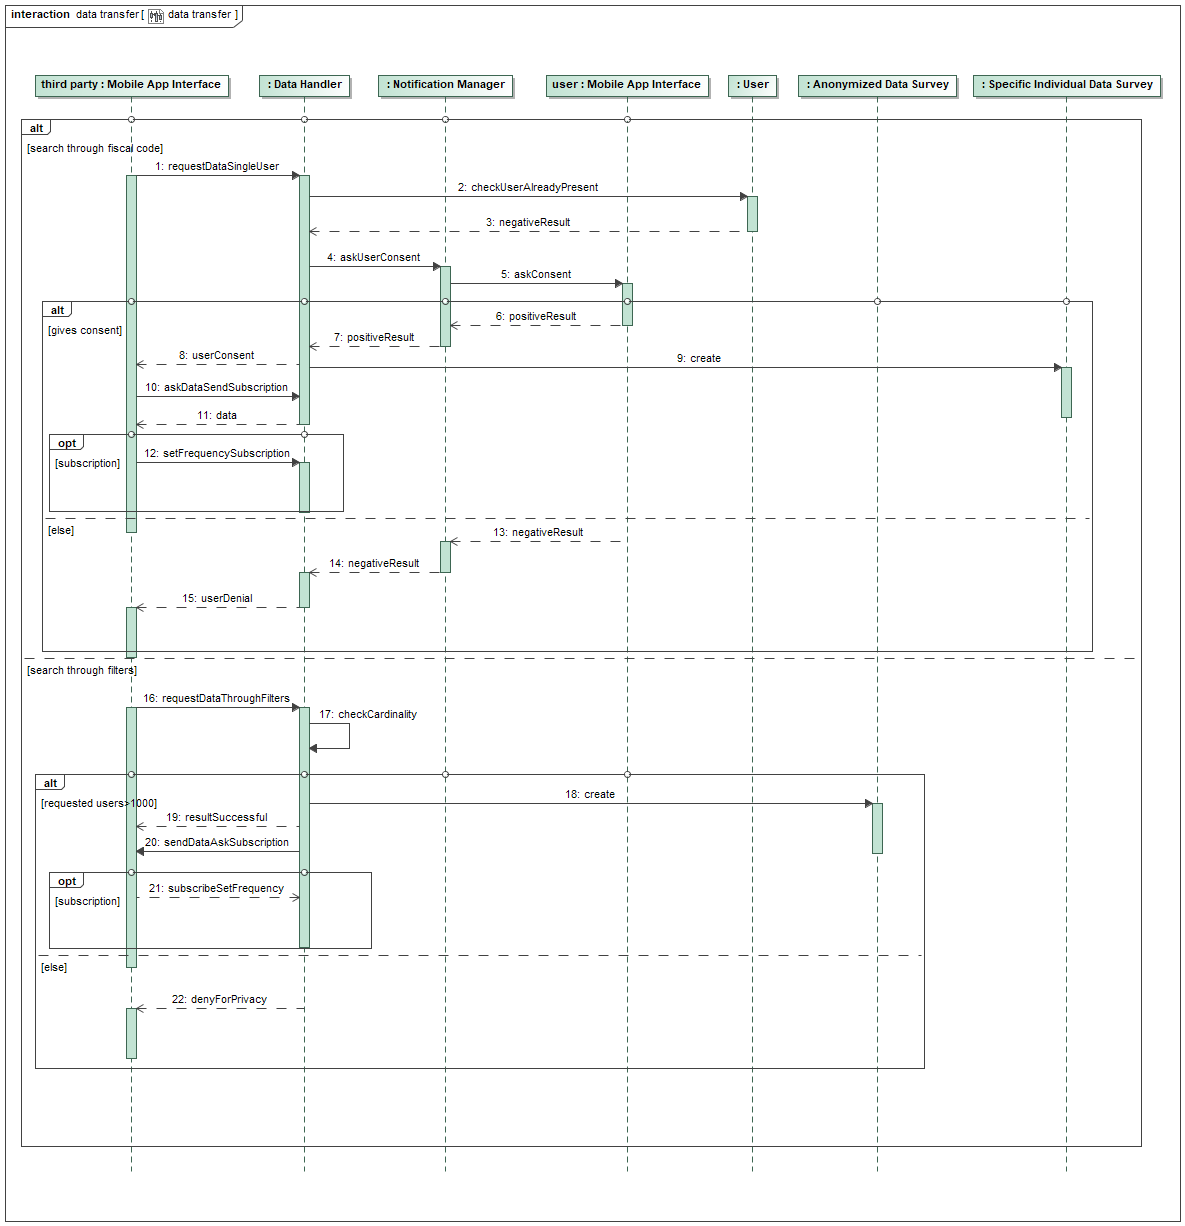
\includegraphics[scale=0.4]{sections/diagrams/data_transfer}
\newline
\captionof{figure}{Sequence diagram of a data request from a third party}
\end{center}

\begin{center}
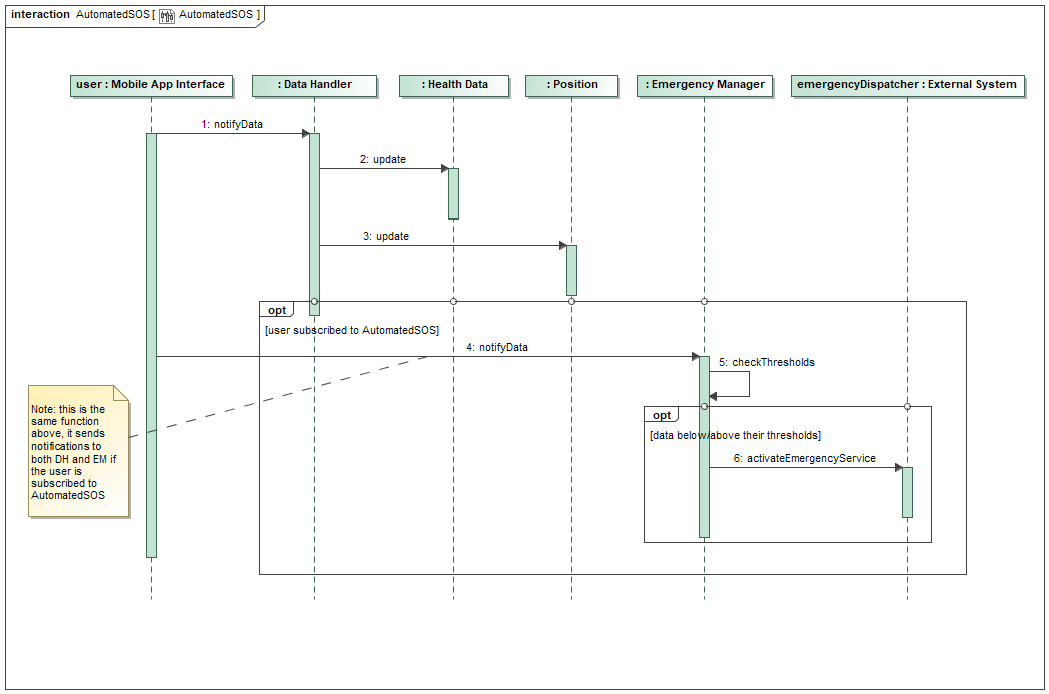
\includegraphics[scale=0.4]{sections/diagrams/AutomatedSOS}
\newline
\captionof{figure}{Sequence diagram of an emergency situation}
\end{center}

\begin{center}
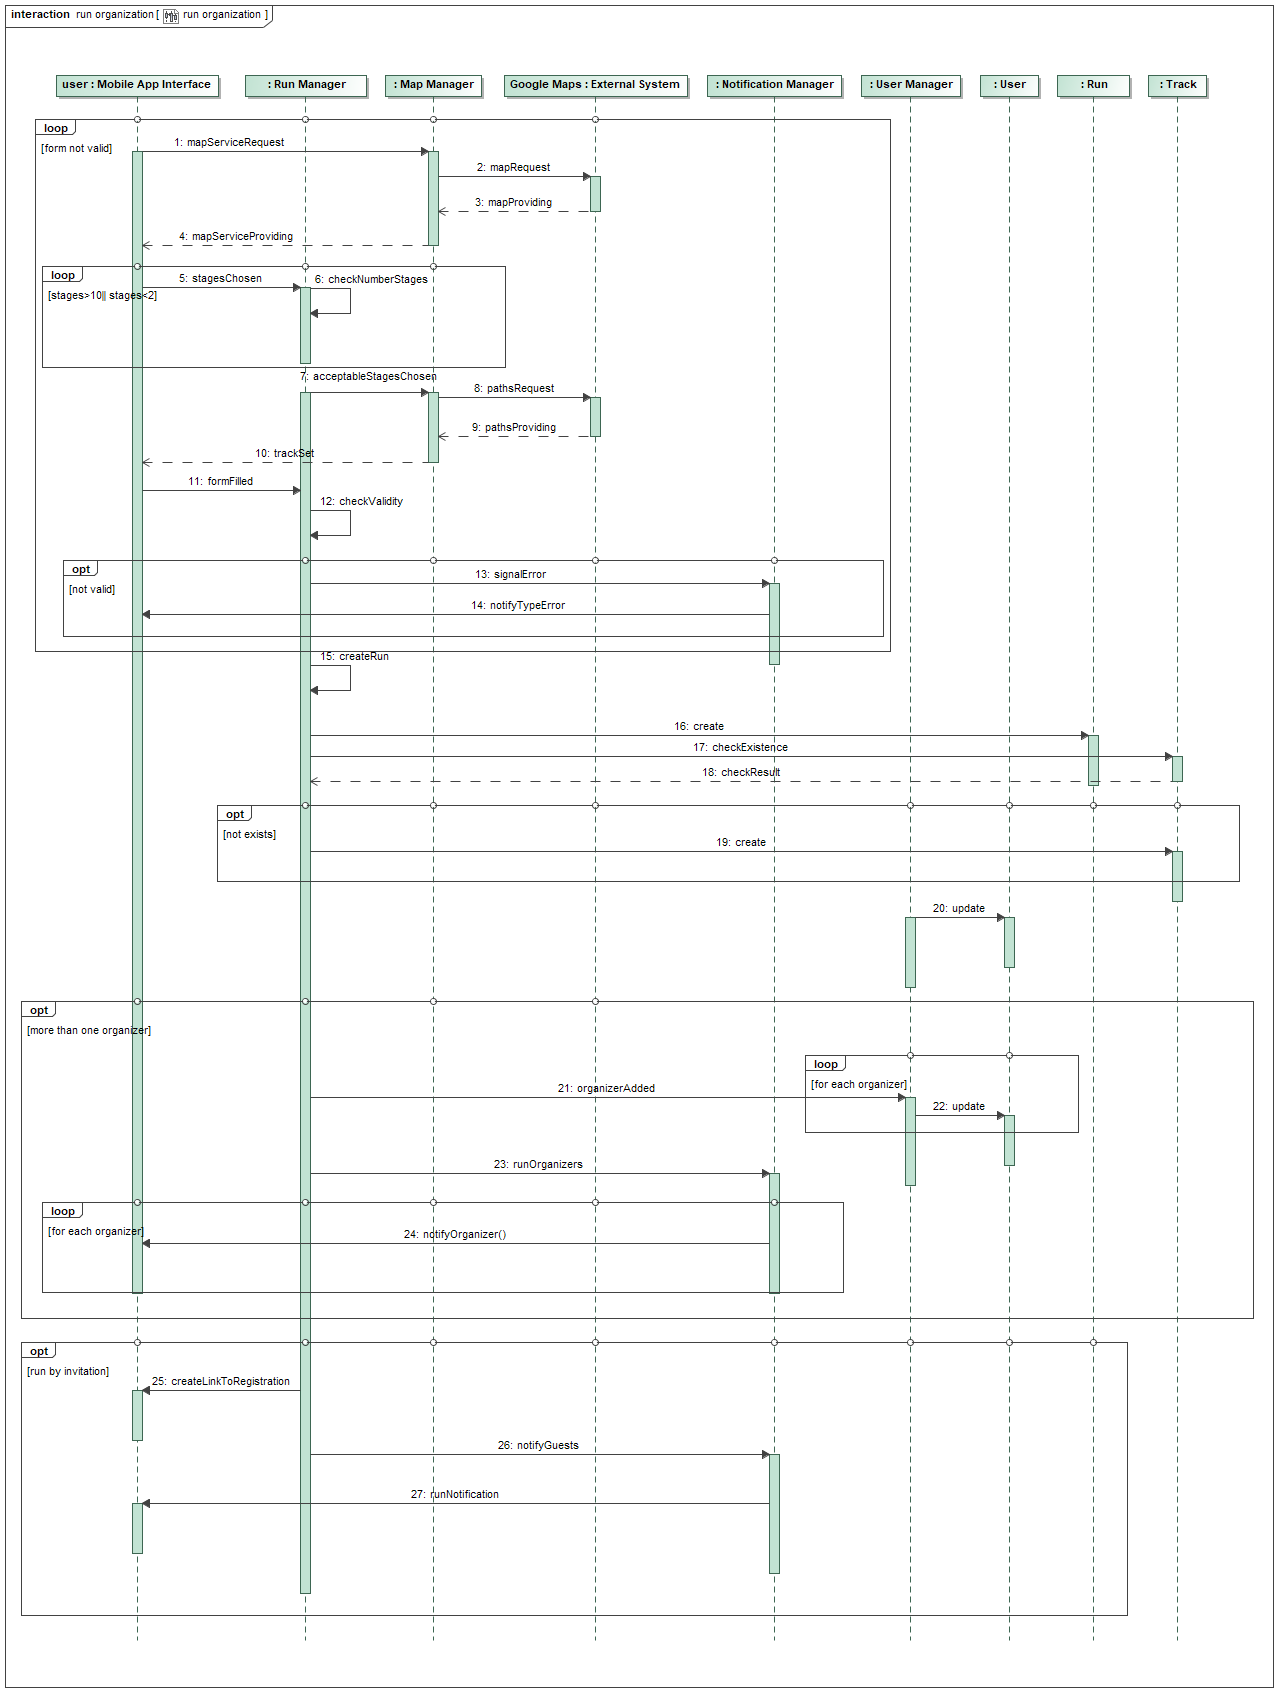
\includegraphics[scale=0.35]{sections/diagrams/run_organization}
\newline
\captionof{figure}{Sequence diagram of a run creation and organization}
\end{center}

\begin{center}
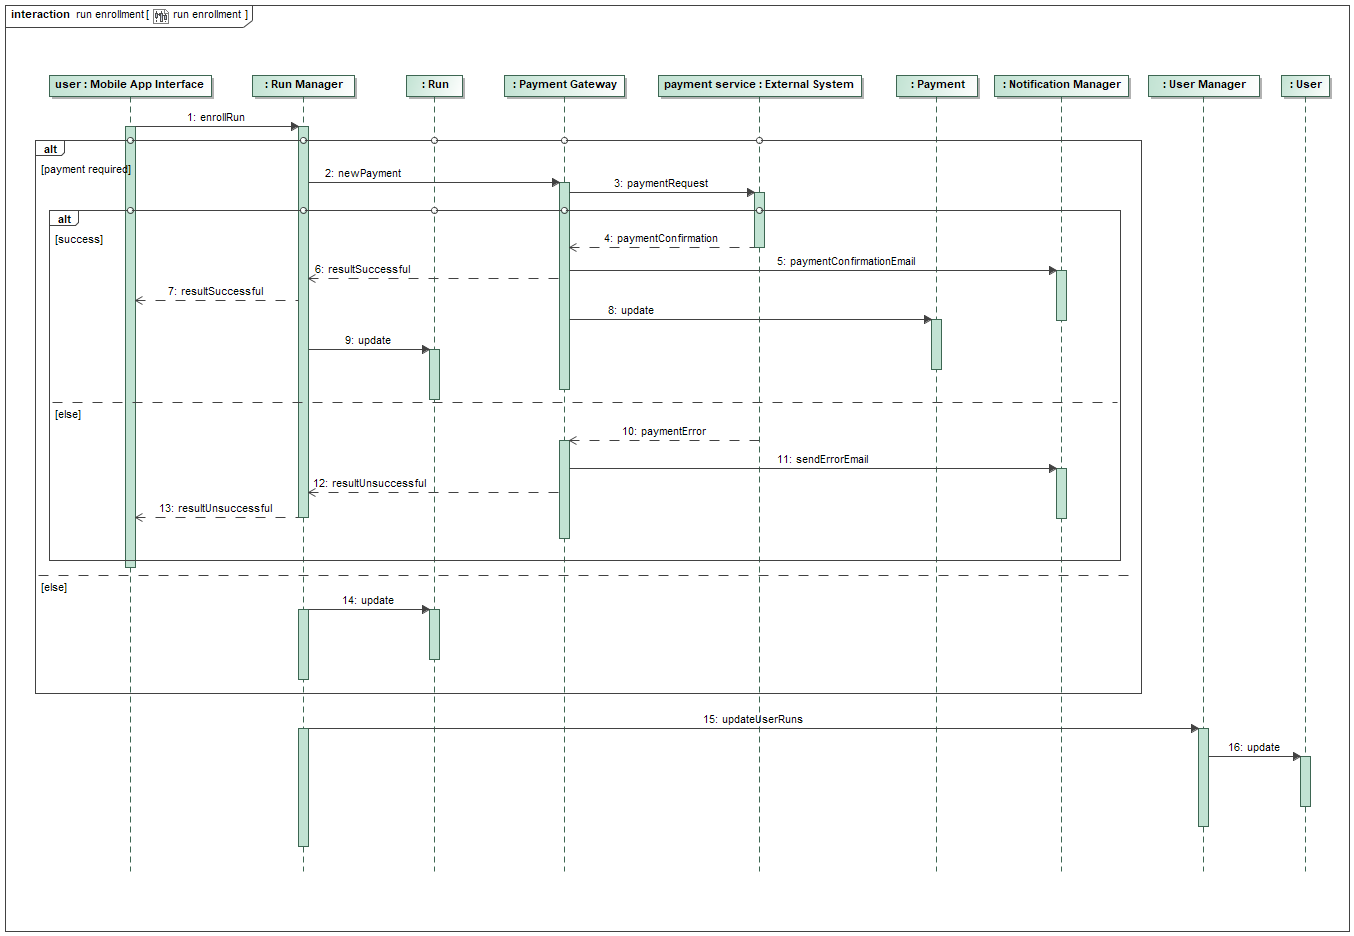
\includegraphics[scale=0.4]{sections/diagrams/run_enrollment}
\newline
\captionof{figure}{Sequence diagram of a run enrollment from a generic user}
\end{center}

\begin{center}
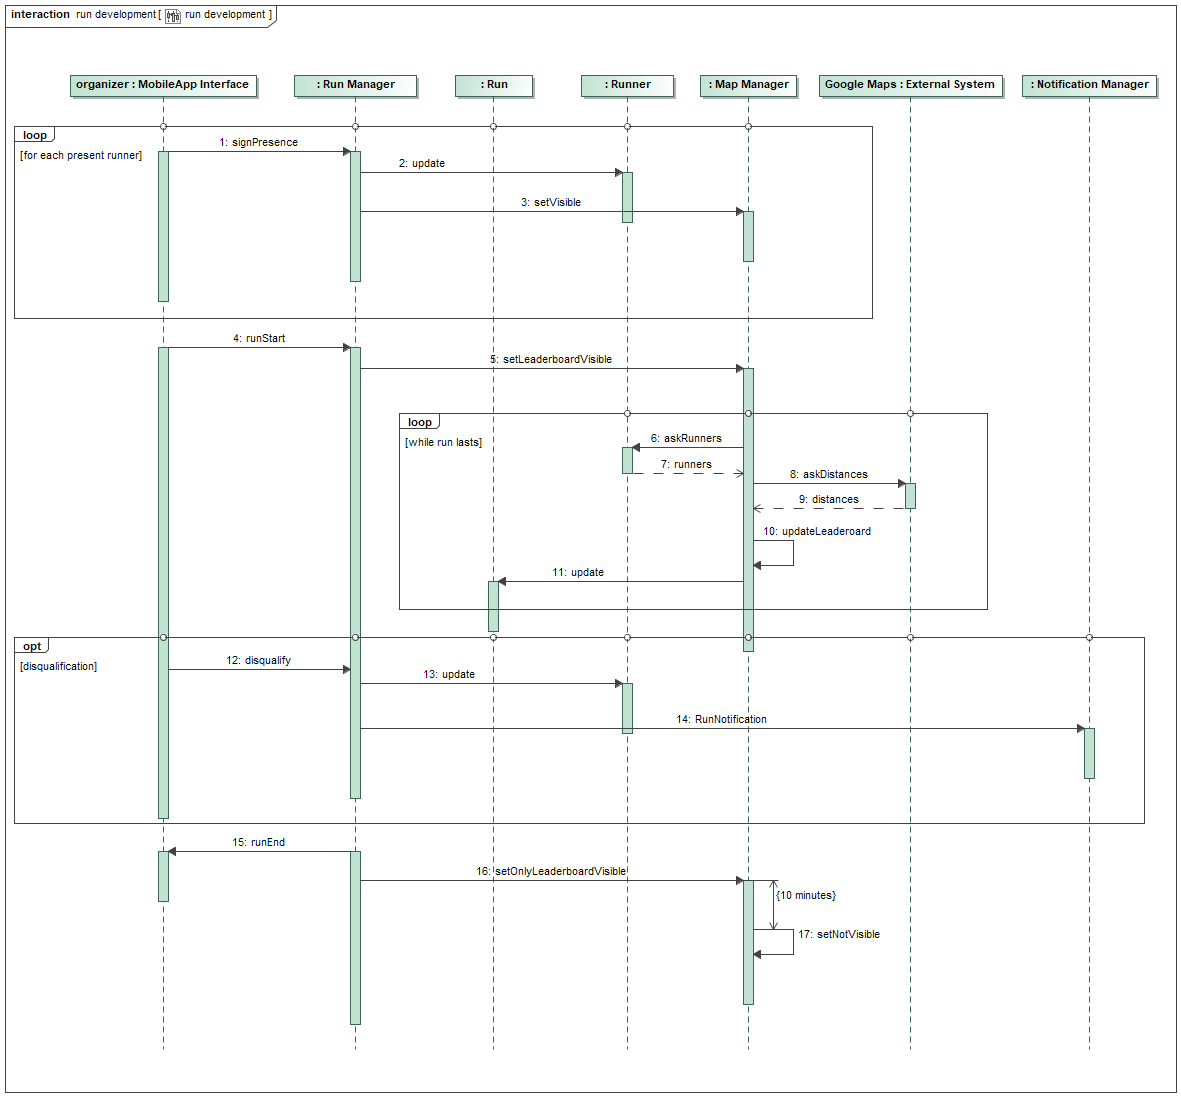
\includegraphics[scale=0.4]{sections/diagrams/run_development}
\newline
\captionof{figure}{Sequence diagram of a run development from its start to its end}
\end{center}

\subsection{Other design decisions}
\subsubsection{Passwords storage}
For security reasons, the user’s password is stored using cryptographic hash functions. In addition to that, the password is not only hashed, but also salted. This is a common security choice since many users reuse passwords for multiple sites and a cyber-attack could jeopardize their sensitive information.
%\end{document}